\documentclass{standalone}

\usepackage{tikz}
\usepackage{pgfplots}

\usetikzlibrary{calc}

\begin{document}
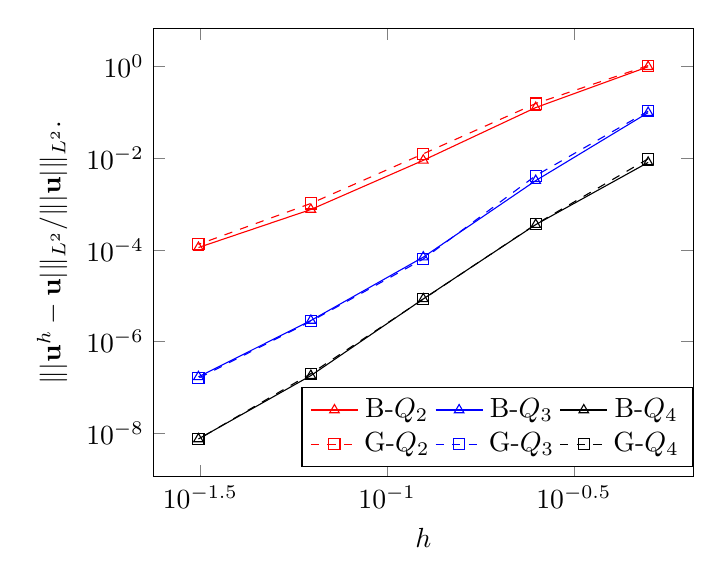
\begin{tikzpicture}
    \begin{loglogaxis}[
        legend columns=3,
        % set `width' and `height' to the desired values
    	legend style={at={(1,.2)}, nodes={scale=1, transform shape}},
        xlabel=$h$,
        ylabel=$\| \vert\mathbf{u}^h-\mathbf{u} \vert \|_{L^2}/\| \vert\mathbf{u} \vert \|_{L^2}$.
    ]

    \addplot [color=red,mark=triangle] plot coordinates {

        (.5,        0.982882)
        (.25,       0.126575)
        (.125,      0.00897637)
        (.0625,     0.000760028)
        (0.03125,   0.000112759)
    };

    
    \addplot [color=blue,mark=triangle] plot coordinates {

        (.5,        0.0983457)
        (.25,       0.00324007)
        (.125,      6.95919e-05)
        (.0625,     2.89258e-06)
        (0.03125,   1.71486e-07)
    };

    \addplot [color=black,mark=triangle] plot coordinates {

        (.5,        0.0080707)
        (.25,       0.000356148)
        (.125,      8.56208e-06)
        (.0625,     1.82399e-07)
        (0.03125,   7.58655e-09)
    };

    \addplot [color=red,mark=square, every mark/.append style={solid}, dashed] plot coordinates {

        (.5,        1.042)
        (.25,       0.155086)
        (.125,      0.0124551)
        (.0625,     0.0010303)
        (0.03125,   0.000131929)
    };

    
    \addplot [color=blue,mark=square, every mark/.append style={solid}, dashed] plot coordinates {

        (.5,        0.105891)
        (.25,       0.00415997)
        (.125,      6.34093e-05)
        (.0625,     2.78257e-06)
        (0.03125,   1.59816e-07)
    };

    \addplot [color=black,mark=square, every mark/.append style={solid}, dashed] plot coordinates {

        (.5,        0.00968295)
        (.25,       0.00036207)
        (.125,      8.44079e-06)
        (.0625,     2.01016e-07)
        (0.03125,   7.49937e-09)
    };


    \logLogSlopeTriangle{0.2}{0.12}{0.06}{4.8}{black};
    \logLogSlopeTriangle{0.2}{0.12}{0.20}{4}{blue};
    \logLogSlopeTriangle{0.2}{0.12}{0.50}{2}{red};

    \legend{B-$Q_2$\\B-$Q_3$\\B-$Q_4$\\G-$Q_2$\\G-$Q_3$\\G-$Q_4$\\}
    \end{loglogaxis}
\end{tikzpicture}

\end{document}
